\documentclass[12pt,A4paper]{article}
\usepackage[left=1.0in,top=1.0in,bottom=1.0in,right=1.0in]{geometry}
\usepackage{blindtext}
\usepackage{sectsty}
\usepackage{blindtext}
\usepackage{graphicx}
\usepackage{subfig}
\usepackage{listings}
\usepackage{color}
\usepackage[utf8]{inputenc}
\usepackage{amsmath}
\usepackage[english]{babel}
\usepackage{setspace}
\usepackage{multicol}
\sectionfont{\fontsize{12}{15}\selectfont}
\subsectionfont{\fontsize{10}{15}\selectfont}
\graphicspath{ {./Figures/} }
\makeatletter
\onehalfspacing
\renewcommand{\@seccntformat}[1]{%
	\ifcsname prefix@#1\endcsname
	\csname prefix@#1\endcsname
	\else
	\csname the#1\endcsname\quad
	\fi}
\addto\captionsenglish{
\renewcommand{\contentsname}
	{Table of Contents}
}
% define \prefix@section
\newcommand\prefix@section{}
\newcommand{\prefix@subsection}{}
\newcommand{\prefix@subsubsection}{}
\renewcommand{\thesubsection}{\arabic{subsection}}
\makeatother
\definecolor{dkgreen}{rgb}{0,0.6,0}
\definecolor{gray}{rgb}{0.5,0.5,0.5}
\definecolor{mauve}{rgb}{0.58,0,0.82}

\lstset{frame=tb,
	language=Matlab,
	aboveskip=3mm,
	belowskip=3mm,
	showstringspaces=false,
	columns=flexible,
	basicstyle={\small\ttfamily},
	numbers=none,
	numberstyle=\tiny\color{gray},
	keywordstyle=\color{blue},
	commentstyle=\color{dkgreen},
	stringstyle=\color{mauve},
	breaklines=true,
	breakatwhitespace=true,
	tabsize=1
}

\begin{document}
	\thispagestyle{empty}
	\begin{center}
		\Huge
		Aer E 261: Final Project \\
		Iowa State University \\
		Jr. JPL \\
		Surveyanator \\
		\vspace{0.25 in}
		
		
		\begin{figure}[!h]
			\centering
			\vspace{0.5 in}
			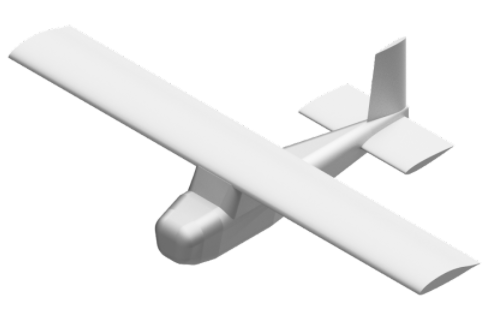
\includegraphics[width=1\textwidth]{IsoCad.png}
			\label{fig:f1}
			\caption{The Surveyanator CAD Model}
		\end{figure}
		\vspace*{\fill}
		\large
		Nicole Buhr, Jeremy Koger, Ellie Mittauer, Justin Pullman, \& Blake Schulte \\
		\vspace{0.25 in}
		Undergraduates in the Department of Aerospace Engineering \\
		Fall 2021 \\
		10 Dec 2021 
		\clearpage
	\end{center}

	\pagenumbering{roman}
	
	\setcounter{page}{2}
	
	\tableofcontents

	\renewcommand\listfigurename{List of Illustrations}
	\listoffigures

	\clearpage
	\pagenumbering{arabic}
	\section{Introduction}
	\hspace{.15 in} The goal of the project is to design an aircraft and predict its performance based on the methods we will be using in AerE 261. The mission is for a craft to survey a given area for threats to human health and/or life. Unmanned aerial vehicles are capable of surveying areas and better mitigating threats. These drones are also capable of observing threats more efficiently than people. The craft will take off from a viable runway far enough away from the affected area. The mission for this aircraft is to take off from makeshift runways and survey land that is inaccessible or hazardous for ground surveying. After take-off, the aircraft would need to be able to ascend to various heights to cruise to the desired destination, then loiter around the desired survey area or areas. While loitering, the aircraft would be documenting areas of land and then flying to other regions to do the same process. All of this would be able to be done autonomously and controlled remotely. After collecting the data, the plane would return to its take-off location to land and return the data. \\
	\indent The Surveyanator will be designed for flying above areas of land or water for geographical, disaster, and search and rescue purposes. It would need to carry various equipment on board, such as photography, radar, Lidar, range finders, and thermal imaging. This craft would serve to aid in search and rescue missions as well as reconnaissance and surveillance.
	

	\clearpage
	\section{Requirements}
	\hspace{.15 in} When starting the design process we set some performance goals that would allow the Surveyanator to complete its mission. To start we wanted to be able to have a range of 100 km to allow for the plane to cruise to the area of interest, survey the area, and return to the launch area. We also wanted the plane to be able to carry different types of equipment. For example cameras, thermal imaging cameras, and other surveying equipment. We estimated that the plane would need to be able to carry at least 20 kg in the payload. The aircraft also needs to have a time in the flight of at least 60 minutes and is capable of operating at a minimum altitude of 1500 meters above the target area. The takeoff and landing distances of the aircraft must also be less than 1000 meters so that its capable of using a variety of airstrips \\
	\indent In addition to the requirements above it also needs to have the ability to take high-altitude photos of disaster areas. Travel at variable speeds for loitering and cruising velocities, specifically low speeds for the sake of taking pictures. 
	

	\clearpage
	\section{Methodology}
	\hspace{.15 in}The design process our team used followed similarly the phases of the design process presented in AerE 261. Using equations derived in class we solved for values about our plane. Our first step was calculating the 2D drag coefficient. Using the mach speed formula (EQ 1\&2) and Reynold’s number formula (EQ 3)we got values to plug into XFLR5 to calculate the 2D drag coefficient for our airfoil, 2D lift slope, alpha at lift equal to 0, and coefficient of lift max. The 2D lift slope, alpha when lift equals zero, and the coefficient of lift was estimated from figure 2. The 2D drag coefficient was estimated from figure 3. \\
	\indent The next thing that we calculated was the 3D drag coefficient. We used the method described in Daniel Raymer’s book “Aircraft Design, A Conceptual Approach” (Raymer, 2012). Using the formulas from the book we were able to calculate the 3D drag coefficients for the wing, fuselage, vertical stabilizer, horizontal stabilizer, and landing gear. This gave us a value of 0.0189 for a whole plane. \\
	\indent After calculating the 3D coefficient of drag we calculated the wing planform area (EQ 4), aspect ratio, (EQ 5) Oswald efficiency (EQ 6), K (EQ 7), and 3D lift slope (EQ 8).\\
	\indent After those calculations, we used the energy needed for the mission to determine the battery weight (EQ 9). Using the calculated weight of the battery we added up the weights (EQ 10) to get similar weight fractions as the Beechcraft Bonanza (EQ 11). Then when changing energy to change the weight of the battery, the weights of the payload, empty weight till the point it was reasonable values and matched the requirements of our plane. One requirement that we had was being able to have a payload of 23 kg. Once we had the total weight of the aircraft we calculated the coefficient of lift at steady level flight (EQ 12). After calculating the coefficient lift needed at steady level flight we could calculate the angle of attack needed for steady level flight (EQ 13). \\
	\indent Now to find the range of our aircraft we started off with finding the $(\frac{C_L}{C_D})_{max}$ (EQ 14) as well as $(\frac{{C_L}^{3/2}}{C_D})_{max}$ (EQ 15). Then using the values above we calculated the endurance (EQ 16), velocity at endurance (EQ 17), range (EQ 18), velocity at max range (EQ 19), and velocity at stall (EQ 20). \\
	\indent Then using a temp vs altitude formula (EQ 21) and density vs altitude (EQ 22), we were able to use the values to calculate the velocity at steady level flight (EQ 23), the power required (EQ 24), the power available (EQ 25), and the power excess (EQ 26), at each altitude. Then we could graph Power vs Altitude shown in figure 4. After calculating the values above we then could calculate the rate of climb (EQ 27), velocity of max rate of climb (EQ 28), the rate of climb max (EQ 29). We then graphed the calculated values to show the rate of climb vs altitude shown in figure 4. We also did a unit conversion of 100 ft per second to meters per second, graphed the service ceiling speed on figure 4 as a horizontal line, and calculated the intersection of the rate of climb max and the service ceiling. \\
	\indent We next calculated the lift at sea level for steady level flight (EQ 30 \& 31). Using the lift calculated we calculated the aerodynamic load limit (EQ 32). For the structural load limits we used values similar to the Cessna 172 of 3.8 g and -1.52 g.  Then using the load limits we calculated pull up radius (EQ 33), pull up turn rate (EQ 34), level turn radius (EQ 35), level turn rate (EQ 36), all for both the aerodynamic limit and structural limit. Then we outputed the highest radius and slowest turning rate for pull up and level turn. This is because the highest radius and slowest turn rate would be using the lowest loading factor. We used the values calculated to make a V-n diagram shown in figure 11. \\
	\indent For takeoff we assumed an obstacle height of 35 meter and for landing a height of 50 meters. For the ground distance for take off we used the ground effect formula (EQ 37), and the ground distance for takeoff (EQ 38). Then using max angle of attack we found the pull up radius at a given airports density. Then we calculated transition height (EQ 39), transition distance (EQ 40), height of the air distance (EQ 41), the air distance (EQ 42), and added all the distances together. This then gave us the total takeoff distance at a given airport. The takeoff distances are shown in figure 5. \\
	\indent For landing calculations we assumed a four degree approach angle. We solved for the flare height (EQ 43) to solve for the height of the approach (EQ 44). Next we solved for the flare distance (EQ 45) and the approach distance (EQ 46).  Next we calculated the ground distance, (EQ 47) then assuming that there was no rolling distance we added  the approach, flare, and ground distances to solve for the landing distance. The landing distances are shown in figure 6. \\
	
	\hspace{.15 in} Most of the assumptions made were ideas presented in class or subjects found when researching aircrafts with similar design and performance. We started by assuming to use the NASA LRN 1015 airfoil for our wings in reference to the RQ-4 Global Hawk unmanned aircraft system. This assumption was made because the military surveillance aircraft has the same mission as the surveyanator. In assuming dimensions for our craft we based the design of the Surveyanator off of the Beechcraft Bonanza shown in figure 9 and figure 10. We made this assumption because it has done similar missions in the past and has the same general form factor. We used a scaling factor of 0.28 at the start of our design process to get physical dimensions. For our weight we decided to scale our aircraft, with the same scaling factor, off of the Cessna 172 Skyhawk because its weight balance made more sense for our mission. Additionally we assumed to leave 23 kg for payload mass because that being 20 percent of our weight fraction makes   sense for our design and 23 kg is enough mass for our surveillance equipment. These were the original assumptions made for weight and design dimensions. These values changed as we performed more calculations and as we learned more in class about aircraft performance, to make sure our mission would be a success. \\
	\indent When we first started the design process we started by scaling everything by a factor of 0.28 based on the Beechcraft Bonanza. This included the weight and size. Once we calculated some of the values like range, endurance, and power required we changed the scaled values to better fit our performance requirements. Each time we entered new equations we tried to change values of our craft to fit our missions. \\
	\indent Once we had our weight, we calculated our CL with that weight and found that our Cl,max was not plausible. To fix this we increased our wingspan (b) to increase our wing planform area (S), to therefore lower our CL value to make sure it is a plausible CL that is well within our Cl,max. Our flight speed remained significantly subsonic and we assumed that our structural weight estimate would allow for the increase in material weight. \\
	\indent Another iteration we made was when we calculated the service ceiling we found that it was a meter off the ground. To fix this we changed the weight estimates while also keeping similar weight fractions. We also found that we extremely overestimated the weight of the surveying equipment. We ended up allotting 26 kg for equipment which gives plenty of room for equipment. \\
	\indent For our propulsion system we assumed that the Aeroexpo electric motor with a high energy dense battery pack would work for our craft because this motor is used in known aircrafts that are currently in production and it fits the thrust requirements. \\
	\indent For our structural load factor we assumed the positive structural load factor of 3.8 and a negative structural load factor of -1.52. These values were given by the company Aeroelectric in reference to the Cessna 172 Skyhawk of which our aircraft design is based.\\

	\clearpage
	\begin{multicols*}{2}
			
	
	\section{Equations}
	\scriptsize
		\begin{equation} \label{eq1} 
			M = \frac{V_\infty }{a_\infty} \\ 
		\end{equation}
		\hrule
		\vspace{0.1 in}
		\begin{equation}
			a_\infty = \sqrt{\gamma R T_\infty} \\
		\end{equation}
		\hrule
		\vspace{0.1 in}
		\begin{equation}
			Re = \frac{\rho_\infty v_\infty c}{\mu_\infty} \\
		\end{equation}
		\hrule
		\vspace{0.1 in}
		\begin{equation}
			s = b * c \\
		\end{equation}
		\hrule
		\vspace{0.1 in}
		\begin{equation}
			AR = \frac{b^2}{s} \\
		\end{equation}
		\hrule
		\vspace{0.1 in}
		\begin{equation}
			e_o = 1.78(1 - 0.045*AR^{0.68}) - 0.64 \\
		\end{equation}
		\hrule
		\vspace{0.1 in}
		\begin{equation}
			k = \frac{1}{\pi e_o AR} \\
		\end{equation}
		\hrule
		\vspace{0.1 in}
		\begin{equation}
			a_{3D} = \frac{a_o}{1 + \frac{57.3 a_o}{\pi e AR}} \\
		\end{equation}
		\hrule
		\vspace{0.1 in}
		\begin{equation}
			W_{battery} = \frac{E_{battery}}{E_{density}} *9.81 \\
		\end{equation}
		\hrule
		\vspace{0.1 in}
		\begin{equation}
			W_{total} = W_{payload} + W_{battery} + W_{empty} \\
		\end{equation}
		\hrule
		\vspace{0.1 in}
		\begin{equation}
			1 = \frac{W_{payload}}{W_{total}} + \frac{W_{empty}}{W_{total}} + \frac{W_{battery}}{W_{total}}\\
		\end{equation}
		\hrule
		\vspace{0.1 in}
		\begin{equation}
			C_L = \frac{W_{total}}{\frac{1}{2} \rho  v_\infty^2  s} \\
		\end{equation}
		\hrule
		\vspace{0.1 in}
		\begin{equation}
			\alpha_{3D\_SLF} = \frac{C_L}{a_{3D}}+\alpha_{L=0} \\
		\end{equation}
		\hrule
		\vspace{0.1 in}
		\begin{equation}
			(\frac{C_L}{C_D})_{max} = \sqrt{\frac{1}{4 K C_{D o}}} \\
		\end{equation}
		\hrule
		\vspace{0.1 in}
		\begin{equation}
			(\frac{{C_L}^{3/2}}{C_D})_{max} = \frac{1}{4} (\frac{3}{K C_{D_o}^{1/3}})^{\frac{3}{4}} \\
		\end{equation}
		\hrule
		\vspace{0.1 in}
		\begin{equation}
			Endurance = (\frac{E_{battery} n_{prop} n_{motor} \sqrt{\rho s}}{\sqrt{2} W_{total}^{1.5}} (\frac{{C_L}^{3/2}}{C_D})_{max}) \div 60 \\
		\end{equation}
		\hrule
		\vspace{0.1 in}
		\begin{equation}
			V_{endurance} = \sqrt{\frac{2}{\rho} * \frac{W_{total}}{s} * \sqrt{\frac{K}{3  CD_o}}} \\
		\end{equation}
		\hrule
		\vspace{0.1 in}
		\begin{equation}
			Range = (\frac{(E_{battery} * n_{motor} * n_{prop})}{W_{total}} * (\frac{C_L}{C_D})_{max}) \div 1000 \\
		\end{equation}
		\hrule
		\vspace{0.1 in}
		\begin{equation}
			V_{maxrange} = \sqrt{\frac{2}{\rho} * \frac{W_{total}}{s} * \sqrt{\frac{K}{CD_o}}}\\
		\end{equation}
		\hrule
		\vspace{0.1 in}
		\begin{equation}
			V_{stall} = \sqrt{\frac{2}{\rho}*\frac{W_{total}}{s}*\frac{1}{Cl_{max}}} \\
		\end{equation}
		\hrule
		\vspace{0.1 in}
		\begin{equation}
			T_{alt} = T_{sea} + a*altitude \\
		\end{equation}
		\hrule
		\vspace{0.1 in}
		\begin{equation}
			\rho_{alt} = \rho_{sea} * {(\frac{T_{alt}}{T_{sea}})}^{\frac{-g}{a*R}-1}\\
		\end{equation}
		\hrule
		\vspace{0.1 in}
		\begin{equation}
			V_{\infty SLF} = \sqrt{\frac{2*W_{total}}{\rho_{alt} * s} * \sqrt{\frac{K}{3CD_o}}}\\
		\end{equation}
		\hrule
		\vspace{0.1 in}
		\begin{equation}
			P_{required} = \frac{1}{2} \rho_{alt} * V_{\infty SLF}^3 * s * CD_o + \frac{2 * K * W_{total}^2}{\rho_{alt}*V_{\infty SLF}*s} \\
		\end{equation}
		\hrule
		\vspace{0.1 in}
		\begin{equation}
			P_{available} = P_{Max} * {\frac{\rho_{alt}}{\rho}}^m \\
		\end{equation}
		\hrule
		\vspace{0.1 in}
		\begin{equation}
			P_{excess} = P_{available} - P_{required} \\
		\end{equation}
		\hrule
		\vspace{0.1 in}
		\begin{equation}
			Rate\_of\_Climb = \frac{P_{excess}}{W_{total}} \\
		\end{equation}
		\hrule
		\vspace{0.1 in}
		\begin{equation}
			V_{Max\_ROC} = \sqrt{{\frac{2*W_{total}}{\rho_{alt}*s}} * \sqrt{\frac{K}{3CD_o}}} \\
		\end{equation}
		\hrule
		\vspace{0.1 in}
		\begin{equation}
			ROC_{Max} = \frac{n_{prop}*P_{available}}{W_{total}} - V_{Max\_ROC} * \frac{1.155}{(\frac{C_L}{C_D})_{max}} \\
		\end{equation}
		\hrule
		\vspace{0.1 in}
		\begin{equation}
			L = C_L * b * q \\
		\end{equation}
		\hrule
		\vspace{0.1 in}
		\begin{equation}
			q = \frac{1}{2} \rho * V_\infty^2 \\
		\end{equation}
		\hrule
		\vspace{0.1 in}
		\begin{equation}
			n_{aero} = \frac{L}{W_{total}} \\
		\end{equation}
		\hrule
		\vspace{0.1 in}
		\begin{equation}
			Pull\_Up_{radius} = \frac{V_\infty^2}{g*(n-1)} \\
		\end{equation}
	\end{multicols*}
	\footnotesize
		\begin{equation}
			Pull\_Up_{rate} = \frac{g*(n-1)}{V_\infty} \\
		\end{equation}
		\hrule
		\vspace{0.1 in}
		\vspace{0.1 in}
		\begin{equation}
			Level\_Turning_{radius} = \frac{V_\infty^2}{g*\sqrt{n^2-1}} \\
		\end{equation}
		\hrule
		\vspace{0.1 in}
		\begin{equation}
			Level\_Turning_{rate} = \frac{V_\infty}{Level\_Turning_{radius}} \\
		\end{equation}
		\hrule
		\vspace{0.1 in}
		\begin{equation}
			Ground\_Effect = \frac{{\frac{16 * h}{b}}^2}{1+{\frac{16 * h}{b}}^2} \\
		\end{equation}
		\hrule
		\vspace{0.1 in}
		\begin{equation}
			s_g = \frac{1.44*W_{total}^2}{g*\rho*Cl_{max}* s * {(Thrust_{Lo} - D_{Lo} - \mu_r*(W_{total}-L_{Lo}))} |_{v=0.7V_{Lo}}} \\
		\end{equation}
		\hrule
		\vspace{0.1 in}
		\begin{equation}
			h_{tr} = R_{pullup} - R_{pullup} * \cos{\theta_{max}} \\
		\end{equation}
		\hrule
		\vspace{0.1 in}
		\begin{equation}
			s_{tr} = R_{pullup} * \sin{\theta_{max}} \\
		\end{equation}
		\hrule
		\vspace{0.1 in}
		\begin{equation}
			h_a = h_{obsticle} - h_{tr} \\
		\end{equation}
		\hrule
		\vspace{0.1 in}
		\begin{equation}
			s_a = \frac{h_a}{\tan{\theta_{max}}} \\
		\end{equation}
		\hrule
		\vspace{0.1 in}
		\begin{equation}
			h_f = R_{pull up} - R_{pull up} * \cos{\theta_f}\\
		\end{equation}
		\hrule
		\vspace{0.1 in}
		\begin{equation}
			h_{a_{land}} = Obs_{hight} - h_f\\
		\end{equation}
		\hrule
		\vspace{0.1 in}
		\begin{equation}
			s_f = R * \sin{\theta_f}\\
		\end{equation}
		\hrule
		\vspace{0.1 in}
		\begin{equation}
			s_{a_{land}} = \frac{h_{a_{land}}}{\tan{\theta_f}}\\
		\end{equation}
		\hrule
		\vspace{0.1 in}
		\begin{equation}
			s_{g_{land}} = \frac{1.69*W_{total}^2}{g*\rho*s*Cl_{max}*(D_{TD} + \mu_r * (W_{total} - L_{TD}))|_{v= 0.7V_{Lo}}}\\
		\end{equation}
		\hrule
		\vspace{0.1 in}

	\normalsize
	
	\clearpage
	\section{Results}
	\begin{figure}[!h]
		\centering
		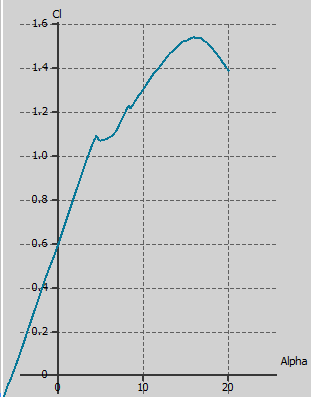
\includegraphics[width=.39\textwidth]{ClAlpha.png}\hspace{0.02 in} \label{fig:f2}
		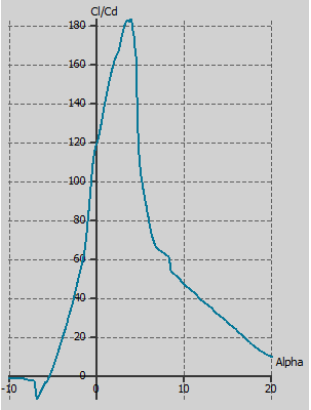
\includegraphics[width=.375\textwidth]{ClCdAlpha.png} \label{fig:f3}
		\caption{Cl vs Alpha (left) \& $\frac{Cl}{Cd}$ vs Alpha (right)}
	\end{figure}
	\begin{figure}[!h]
		\centering
		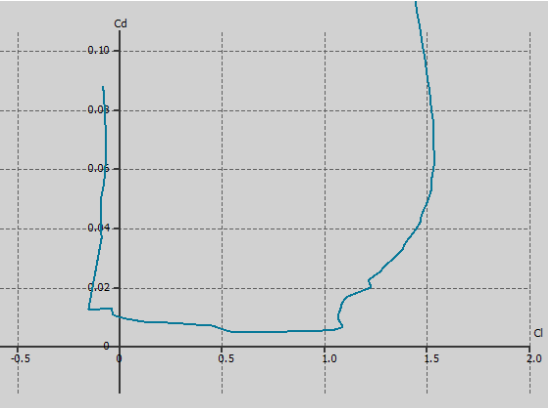
\includegraphics[width=.6\textwidth]{CdCl.png} \label{fig:f4}
		\caption{Cd vs Cl}
	\end{figure}
	\begin{figure}[!h]
		\centering
		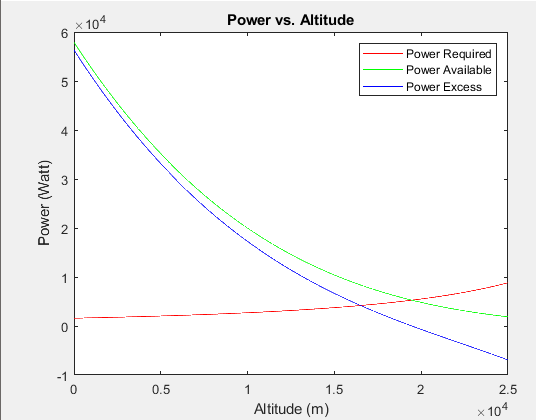
\includegraphics[width=.375\textwidth]{PowerVAltitude.png}\hspace{0.02 in} \label{fig:f5}
		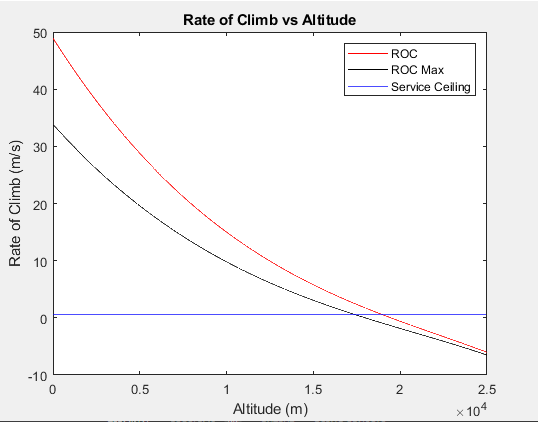
\includegraphics[width=.375\textwidth]{RateofClimb.PNG} \label{fig:f6}
		\caption{Power vs Altitude (left) \& Rate of Climb vs Altitude (right)}
	\end{figure}
	\begin{figure}[!h]
		\centering
		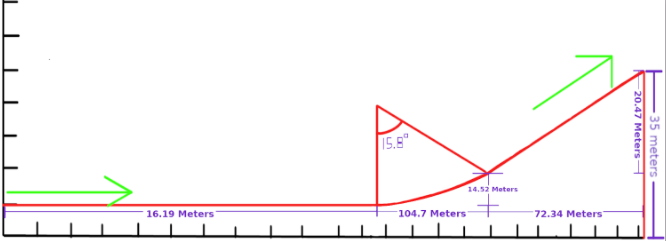
\includegraphics[width=.75\textwidth]{TakeOff.PNG} \label{fig:f7}
		\caption{Takeoff}
	\end{figure}
	\begin{figure}[!h]
		\centering
		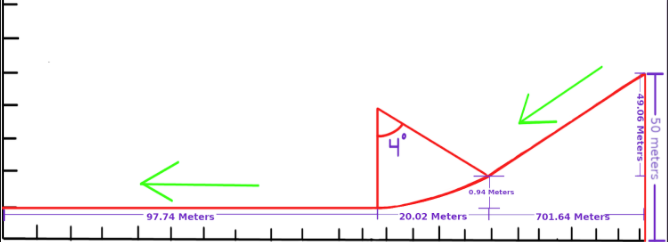
\includegraphics[width=.75\textwidth]{Landing.PNG} \label{fig:f8}
		\caption{Landing}
	\end{figure}
	\begin{figure}[!h]
		\centering
		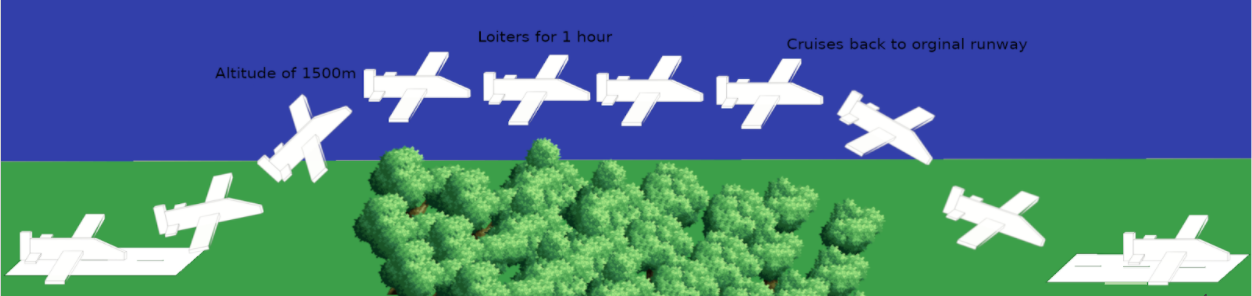
\includegraphics[width=.75\textwidth]{Mission.PNG} \label{fig:f9}
		\caption{Mission Overview}
	\end{figure}
	\begin{figure}[!h]
		\centering
		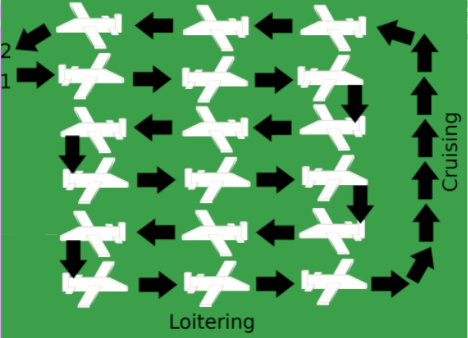
\includegraphics[width=.5\textwidth]{Holding.PNG} \label{fig:f10}
		\caption{Survey Pattern}
	\end{figure}
	\begin{figure}[!h]
		\centering
		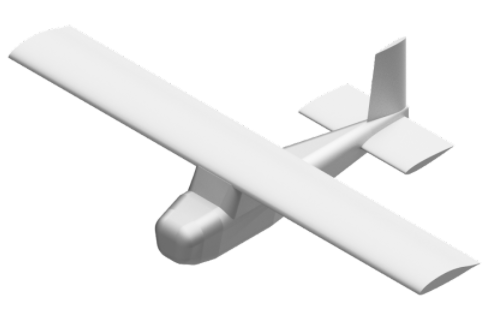
\includegraphics[width=.4\textwidth]{IsoCad.PNG}\hspace{.2 in} \label{fig:f11}
		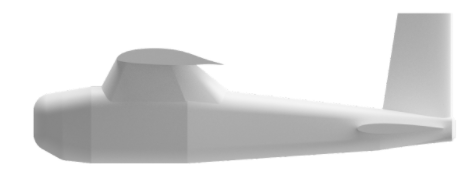
\includegraphics[width=.4\textwidth]{side.PNG} \label{fig:f12}
		\caption{CAD Model Iso view (left) \& Side view (right)}
	\end{figure}
	\begin{figure}[!h]
		\centering
		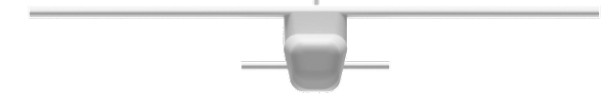
\includegraphics[width=.6\textwidth]{Front.PNG} \label{fig:f13}
		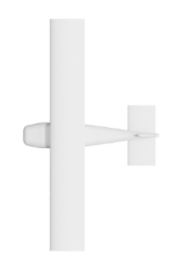
\includegraphics[width=.2\textwidth]{Top.PNG} \label{fig:f14}
		\caption{CAD Model Front view (left) \& Top view (right)}
	\end{figure}
	\begin{figure}[!h]
		\centering
		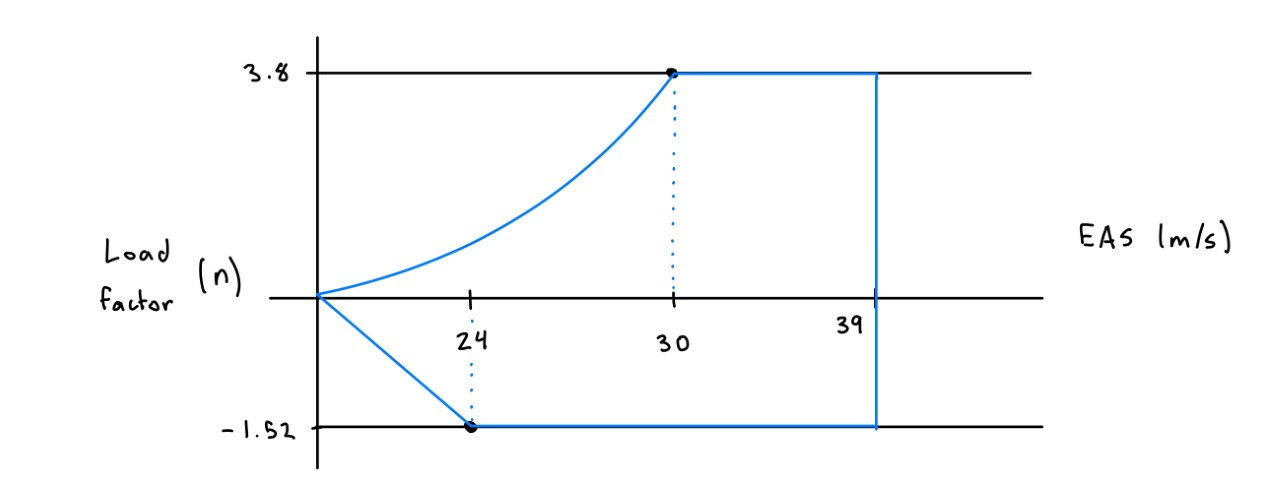
\includegraphics[width=.6\textwidth]{VN.JPG} \label{fig:f17}
		\caption{V-N Diagram}
	\end{figure}
	\begin{figure}[!h]
		\centering
		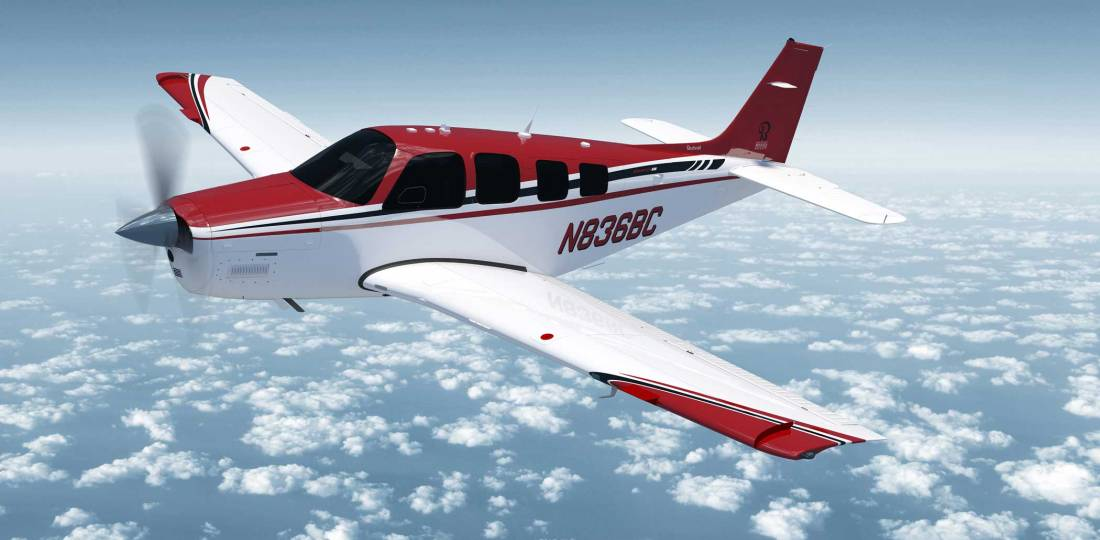
\includegraphics[width=.6\textwidth]{beechcraft.JPG} \label{fig:f15}
		\caption{Beechcraft Bonanza}
	\end{figure}
	\begin{figure}[!h]
		\centering
		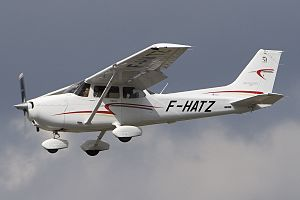
\includegraphics[width=.6\textwidth]{cessna.JPG} \label{fig:f16}
		\caption{Cessna}
	\end{figure}
	
	\clearpage
	\section{Discussion}
	 \hspace{.15 in}The results we got after a few iterations of flight speed and overall weight of the craft seem reasonable. With an endurance of 105.5 minutes and a range of 168.7 kilometers, our craft is able to complete its mission and is within a reasonable range of other like-sized drones. The takeoff and landing distances are also reasonable values with the craft being able to take off in 193 meters and land in 820 meters, with actual runway use being only 16 and 97 meters respectively. These values easily allow us to complete our mission parameters and are within reason for a craft of our size and weight. The craft flies between 20 and 30 meters per second with a stall velocity of 19.8 meters per second. \\
	\indent The one value that doesn’t make much sense is our service ceiling. Our script tells us that our service ceiling is 17502 meters which is well above what an electric prop-driven craft should be able to achieve. Our mission altitude is only 1500 meters, so while being able to achieve this easily is good news, a value 11 times higher is suspicious. \\
	\indent We assumed that we would be flying at a relatively low altitude (1500 meters) and at lower speeds (30 m/s), these assumptions affect nearly every equation used so may have an impact if the craft finds itself flying faster or higher. \\
	\indent We had some issues as we continued to add new sections to the MatLab script. We had made some assumptions in the beginning while we were still figuring out the individual equations. We also made some mistakes in the early equations which carried through to the later additions giving us numbers far from what they should have been. 
	We started by using a Beechcraft bonanza model for weight and proportions and scaling it down by a third. We substituted the wing design of a Global Hawk military drone (Figure 12). After a few weeks, we realized our weight was too high for an electric motor to get any usable range or speed. We switched our weight estimate scale down from the Beechcraft Bonanza to the Cessna 172 Skyhawk (Figure 13). This got us closer to our desired range and speed, but we were still too heavy, so we scaled down our payload weight from a couple of hundred pounds to fifty pounds. We thought this would be plenty for a camera or radar system. Cutting this weight also allowed us to use less energy to go the same distance and speed, so we were able to reduce the battery weight as well. After making these changes our numbers started making more sense. 
	
	\clearpage
	\section{Conclusion}
	\hspace{.15 in}In the age of information, there is no reason why there cannot be detailed surveillance over any area. Our objective was to create an aircraft for search and rescue, surveillance, and reconnaissance missions. We achieved our goals by creating an unmanned aerial vehicle that has thermal, Lidar, range finders, and visible light capture capabilities. Our aircraft is capable of landing and taking off from makeshift runways to access dangerous air space where sending pilots is too risky.  The aircraft is able to reach the desired altitudes for cruising at various heights. This allows the aircraft to cruise to its destination and survey an area. While loitering, the aircraft can use the surveillance equipment to complete its mission. Our objective cruise altitude was originally set to 1500 meters to get adequate photographs of disaster areas and we were able to stay true to that target value throughout the design process. During the course of designing the craft, we had to change the concept in order to better suit the mission while still meeting the requirements from the initial design of the aircraft. Some of these changes were to make the craft lighter and decrease the size of the battery in order to increase our flight time. This required us to decrease the cruise velocity to compensate for the reduced power output. Through the various design iterations, we were also able to increase the efficiency of the propulsion system, therefore, increasing our endurance by almost double for more wiggle room in flight to accomplish the mission. The initial range of the aircraft from takeoff to landing had to be shortened in order to remain consistent with the reduced power of the propulsion system. Through the reduction of the propulsion system as well we successfully brought the gross takeoff weight down to approximately 200 lbs. While its intended use is search and rescue and reconnaissance, the Surveyanator is a versatile craft. Our aircraft features state-of-the-art photographic technology for the long-range detection of targets. Our onboard surveillance system is perfect for keeping track of targets around the clock.
	\clearpage
	\section{References}
	\sloppy
	“Rex-90 - Ulm Electric Motor by MGM Compro: Aeroexpo.” The B2B Marketplace for Aeronautical Equipment, https://www.aeroexpo.online/prod/mgm-compro/product-171210-31063.html. \\ \\
	http://www.aeroelectric.com\/Reference\_Docs\/Cessna\/cessna-misc\/C172\_Performance-Figures\_\_from\_RSV\_Cessna\_Training\_Manual.pdf \\ \\
	Raymer, D. P. (2012). Determination of CD,0 Using the Component Build Up Method. In Aircraft design: A conceptual approach. essay, AIAA. \\ \\
	Phelps, Mark. “Beechcraft Honors U.S. Bonanza Society with Custom G36.” Aviation International News, 27 July 2016, https://www.ainonline.com/aviation-news/general-aviation/2016-07-27/beechcraft-honors-us-bonanza-society-custom-g36. \\ \\
	“Cessna 172.” Wikipedia, Wikimedia Foundation, 1 Dec. 2021, https://en.wikipedia.org/wiki/Cessna\_172. \\
	\clearpage
	\section{Code}
	\begin{center}
	Link to Inputs Document: https://docs.google.com/spreadsheets/d/1mX9oFI3Zd5SyJR2twwYRWJ417U7gUv60qco82aeOLdE/\\edit?usp=sharing \\
	\begin{figure}[!h]
		\centering
		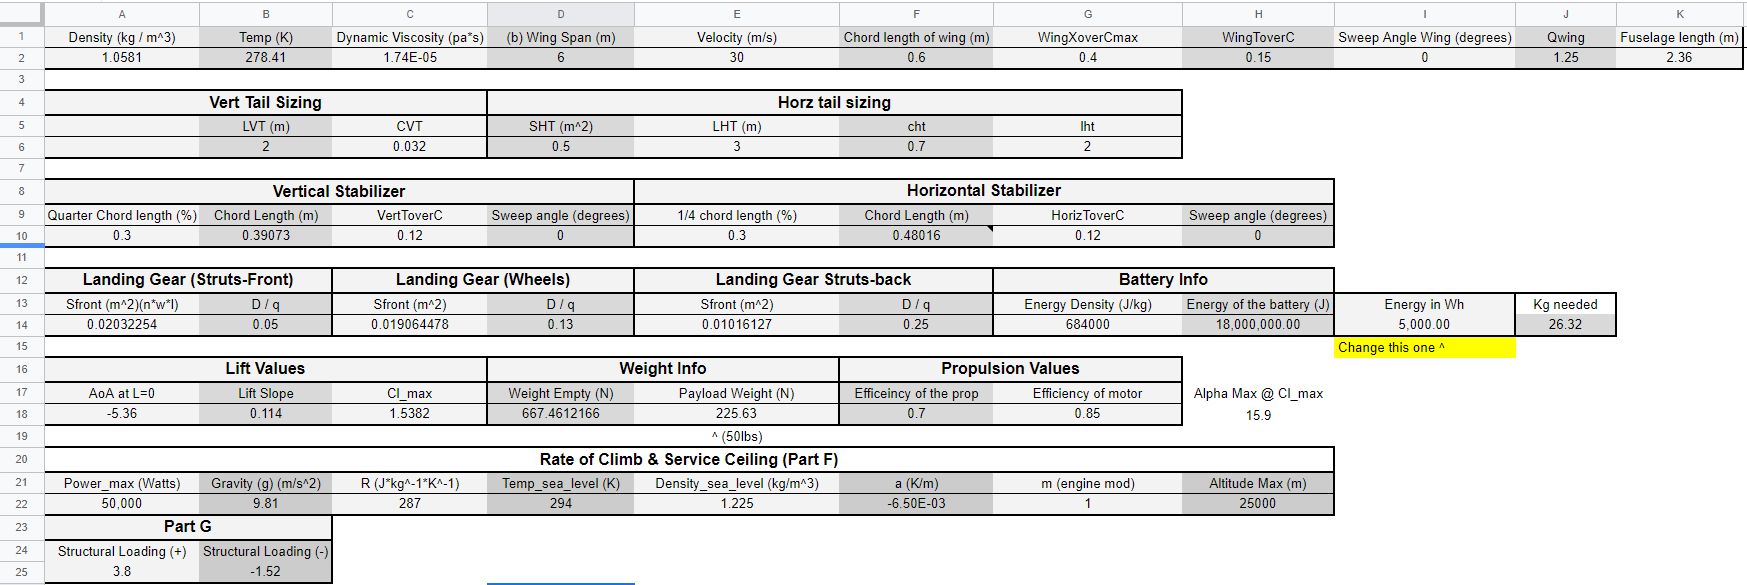
\includegraphics[width=1\textwidth]{Inputs.PNG} \label{fig:f15}
		\caption{Google Sheets Inputs}
	\end{figure}
	\end{center}
	\begin{lstlisting}
		clear,clc,clf
		%AerE 261
		%Jr.JPL Blake, Ellie, Jeremy, Justin, Nicole
		%Surveyanator
		%scaling factor 0.28:1 to the bonanza
		%based of Beechcraft Bonanza and Cessna 172
		
		
		inputs = GetGoogleSpreadsheet('1mX9oFI3Zd5SyJR2twwYRWJ417U7gUv60qco82aeOLdE');
		inputs = str2double(inputs);
		inputs = num2cell(inputs);
		%Import Vars from Spreadsheet --->
		[density, temp, dynamicViscosity, wingSpan, velocity, wingChord, wingXOverC, wingTOverC, wingSweepAngle, Qwing, fuselageLength] = inputs{2,:};
		[LVT, CVT, LHT, cht, lht] = inputs{6,2:7};
		[quarterChordVertStab, chordVertStab, vertTOverC, vertSweepAngle, quarterChordHorzStab, chordHorzStab, horzToverC, horzSweepAngle] = inputs{10,1:8};
		[frontStruts_Sfront, frontStruts_dOverq, wheel_Sfront, wheel_dOverq, backStrut_Sfront, backStrut_dOverq, E_density, E_battery] = inputs{14,1:8};
		[alat0, anot, Cl_max, W_e, W_p, n_prop, n_motor] = inputs{18,1:7};
		[Power_Max, g, R, Tsea, density_sea, a, m, altitude_max] = inputs{22,1:8};
		[n_Strut_pos, n_Strut_neg] = inputs{25,1:2};
		
		%General Calculations ---->
		Mach_val = Mach(velocity, temp); %meters/second
		
		%Main Wing Calcs -->
		Swing = wingSpan*wingChord; %(meters^2)
		ReWing = Reynolds(density,velocity,dynamicViscosity,wingChord);
		cfWing = FrictionCoefficient(ReWing,Mach_val);
		FFWing = FormFactor(wingXOverC,wingTOverC,wingSweepAngle,Mach_val);
		wingSWetted = (1.977+0.52*wingTOverC)*Swing; %(m^2)
		cd_o_Wing = cfWing*FFWing*(wingSWetted/Swing)*Qwing;
		
		%Fuselage Calcs -->
		fuselageAreaFront = 0.44432 * 0.58674; %[meters^2] %Taken from cad max width and height
		f = fuselageLength/(sqrt((4/pi)*fuselageAreaFront)); 
		ffFuse = 0.9 + (5/(f^1.5))+(f/400);
		ReFuse = Reynolds(density,velocity,dynamicViscosity,fuselageLength);
		fuselageAreaTop = 0.44432 * 2.33807; %[m^2] Taken from cad general over estimate
		sWettedFuse = 3.4*((fuselageAreaTop + fuselageAreaFront)/2);
		cfFuse = FrictionCoefficient(ReFuse,Mach_val);
		cd_o_Fuse = cfFuse*ffFuse*1*(sWettedFuse/Swing);
		
		%Vert tail sizing calcs -->
		[svt] = TailVertCoefficient(CVT,LVT,wingSpan,Swing);
		
		%Horz tail sizing calcs -->
		Cavg = Swing/wingSpan;
		[sht] = TailHorizCoefficient(cht,lht,Cavg,Swing);
		
		%Vertical Stabilizer calcs -->
		ReVert = Reynolds(density,velocity,dynamicViscosity,chordVertStab);
		cfVert = FrictionCoefficient(ReVert,Mach_val);
		ffVert = FormFactor(quarterChordVertStab,vertTOverC,vertSweepAngle,Mach_val);
		sWettedVert = CVT/Swing; %(m^2)
		cd_o_Vert = cfVert*ffVert*(sWettedVert/Swing)*1.05; %Swing was 2.15, not concurrent with CD0-estimateion.pdf
		
		%Horizontal Stabilizer calcs -->
		ReHoriz = Reynolds(density,velocity,dynamicViscosity,chordHorzStab);
		
		cfHoriz = FrictionCoefficient(ReHoriz,Mach_val);
		ffHoriz = FormFactor(chordHorzStab,horzToverC,horzSweepAngle,Mach_val);
		sWettedHoriz = cht/Swing; %meters^2
		cd_o_Horz = cfHoriz*ffHoriz*(sWettedHoriz/Swing)*1.05; %Swing was 2.15, not concurrent with CD0-estimateion.pdf
		
		%Landing gear struts (front 2) calcs -->
		cd_o_landF = frontStruts_dOverq*(frontStruts_Sfront/Swing);
		
		%Landing gear struts (back 1)  calcs -->
		cd_o_landB = backStrut_dOverq*(backStrut_Sfront/Swing);
		
		%Landing Gear Wheels (3 wheels) calcs -->
		cd_o_wheels = wheel_dOverq*(wheel_Sfront/Swing);
		
		%Drag buildup calcs -->
		CD_o = cd_o_Wing + cd_o_Fuse + cd_o_Vert + cd_o_Horz + cd_o_landB + cd_o_landB + cd_o_wheels;
		
		%Lift calculations -->
		AR = (wingSpan^2)/Swing;
		e_o = 1.78*(1-0.045*(AR^0.68))-0.64; %Unitless
		K = 1/(pi*e_o*AR);
		a3D = anot/(1+((57.3*anot)/(pi*0.7*AR)));
		
		%Battery Calculations -->
		batteryWeight = (E_battery/E_density)*9.81; %(N)
		
		%Cl & CL calcs -->
		W_total = W_e + W_p + batteryWeight; %(Newtons)
		CLift = W_total / (0.5 * density * (velocity^2) * Swing);
		
		%Weight Fraction Calcs -->
		frac_W_e = W_e/W_total;
		frac_W_p = W_p/W_total;
		frac_W_f = batteryWeight/W_total;
		
		%AoA @SLF
		alpha3D_SLF = (CLift/a3D)+alat0; %derived from CL = a(alpha - alpha_L=0)
		
		%Range calculations -->
		CLoCD_max = sqrt(1/(4*K*CD_o)); %Should this be under a squareroot?
		CLoCD_3half_max = 0.25*(((3)/(K*CD_o^(1/3)))^(3/4));
		endurance = (((E_battery * n_prop * n_motor * sqrt(density * Swing)) / (sqrt(2) * (W_total^(1.5))))* CLoCD_3half_max )/60; %in seconds /60 --> min
		V_endurance = sqrt(((2/density) * (W_total/Swing)) * sqrt(K/(3 * CD_o)));
		range = (((E_battery * n_motor * n_prop) / W_total) * CLoCD_max) / 1000; %km
		V_maxrange = sqrt(((2/density) * (W_total/Swing)) * sqrt(K/CD_o)); %m/s
		V_stall = sqrt((2/density)*(W_total/Swing)*(1/Cl_max));
		
		%Part E
		altitude= 0:1:altitude_max; %meters
		
		Temp_alt = Tsea+a.*(altitude); %Kelvin
		
		density_alt = density_sea.*(Temp_alt/Tsea).^((-g/(a*R))-1); %kg/m^3
		
		v_infin_SLF = (((2*W_total)./(density_alt.*Swing).*(K./(3*CD_o)).^(.5)).^(0.5)); %m/s
		Power_req = .5.*density_alt.*((v_infin_SLF).^(3)).*Swing*CD_o+((2*K*((W_total)^(2)))./(density_alt.*v_infin_SLF*Swing)); %watts
		Power_avail = Power_Max.*((density_alt./density).^(m)); %watts
		Power_excess = Power_avail-Power_req; %watts
		
		plot(altitude,Power_req,'color','r')
		hold on
		plot(altitude,Power_avail,'color','g')
		hold on
		plot(altitude,Power_excess,'color','b')
		hold off
		legend('Power Required','Power Available','Power Excess')
		xlabel('Altitude (m)')
		ylabel('Power (Watt)')
		title('Power vs. Altitude')
		
		ROC = Power_excess./W_total; %m/s
		VMax_ROC = (((2*W_total)./(density_alt.*Swing)).*((K/(3*CD_o))^(.5))).^(0.5); %m/s
		ROC_Max = ((n_prop.*Power_avail)./(W_total))-VMax_ROC.*((1.155)./(CLoCD_max)); %m/s
		Service_ceiling = 100/(60*3.28084); %m/s
		
		figure()
		plot(altitude,ROC,'color','r')
		hold on
		plot(altitude,ROC_Max,'color','k')
		hold on
		yline(Service_ceiling,'color','b')
		hold off
		xlabel('Altitude (m)')
		ylabel('Rate of Climb (m/s)')
		legend('ROC','ROC Max','Service Ceiling')
		title('Rate of Climb vs Altitude')
		
		% Finding the altitude where ROC max equals the service ceiling
		Intersections=find(abs(ROC_Max - Service_ceiling)<=(0.002));
		
		SC=altitude(Intersections); %Service ceiling in meters
		Height_service = mean(SC);
		
		%Part G
		%Pull up
		q = (0.5)*(density)*(velocity^2);
		Lift = CLift * wingSpan * q;
		n_Aero = Lift / W_total;
		[PU_radius_Aero,PU_turnRate_Aero,LT_radius_Aero,LT_turnRate_Aero] = TurningRad_andRate (V_endurance,g,n_Aero);
		[PU_radius_Strut,PU_turnRate_Strut,LT_radius_Strut,LT_turnRate_Strut] = TurningRad_andRate (V_endurance,g,n_Strut_pos);
		[PU_radius,PU_turnRate,LT_radius,LT_turnRate] = LoadLimitedTurning (PU_radius_Aero,PU_turnRate_Aero,LT_radius_Aero,LT_turnRate_Aero,PU_radius_Strut,PU_turnRate_Strut,LT_radius_Strut,LT_turnRate_Strut);
		vel_manuv = sqrt(((2*n_Strut_pos)/(density*Cl_max))*(W_total/Swing));
		
		
		
		%Part H
		Cl_at0 = 0.6;
		density_runway = 1.225; %kg/m^3 %able to change density based of airport altitude
		mu_r = 0.4; %Hard turf or dry concrete
		V_stall_runway = sqrt((2/density)*(W_total/Swing)*(1/Cl_max)); %m/s
		
		%takeoff
		obs_h = 35; %meters
		V_Lo = 1.2*V_stall_runway; %m/s
		Thrust_Lo = Power_Max/V_Lo; %Newtons %Max thrust
		L_Lo = 0.5*density_runway*((0.7*V_Lo)^2)*Swing*Cl_at0; %Newtons 
		groundHeight = 0.5; %meters %JP - Subject to change, just an estimate
		groundEffect = ((16*groundHeight/wingSpan)^2)/(1+(16*groundHeight/wingSpan)^2);
		D_Lo = 0.5*density_runway*((0.7*V_Lo)^2)*Swing*(CD_o+groundEffect*K*(Cl_at0^2)); %Newtons
		s_g = (1.44*W_total^2)/(g*density_runway*Cl_max*Swing*(Thrust_Lo - D_Lo - mu_r*(W_total-L_Lo))); %meters
		
		max_theta = 15.8; %degs %min angle to get over obsticle
		R_pullup = (1.44*(V_stall_runway^2))/(0.15*g); %meters
		h_tr = R_pullup-R_pullup*cosd(max_theta); %meters
		s_tr = R_pullup*sind(max_theta); %meters
		h_a = obs_h-h_tr; %meters
		s_a = h_a/tand(max_theta); %meters
		
		s_takeoff = s_g+s_tr+s_a; %meters
		
		
		%landing
		landobs_h = 50; %meters
		theta_f = 4; %deg
		h_f = R_pullup-R_pullup*cosd(theta_f); %meters
		s_f = R*sind(theta_f); %meters
		h_aland = landobs_h-h_f; %meters
		s_aland = h_aland/tand(theta_f); %meters
		
		V_TD = 1.15*V_stall_runway; %m/s 
		L_TD = 0.5*density_runway*((0.7*V_TD)^2)*Swing*Cl_at0; %Newtons
		D_TD = 0.5*density_runway*((0.7*V_TD)^2)*Swing*(CD_o+K*(Cl_at0^2)); %Newtons
		s_gland = (1.69*W_total^2)/(g*density_runway*Swing*Cl_max*(D_TD+mu_r*(W_total-L_TD))); %meters
		
		s_landing = s_gland+s_f+s_aland; %meters
		
		%Presentation
		Wingload = W_total/Swing;
		LoverD = CLift/(CD_o+K*(CLift^2));
		ToverW = (Power_Max/30)/W_total;
		
		
		%Displaying values of interest
		fprintf('CL = %g*(alpha-(%g))\n',a3D,alpha3D_SLF) %3Dlift equation
		fprintf('Aspect Ratio = %g\n',AR)
		fprintf('Planform Area = %g m^2\n',Swing)
		fprintf('Mach_val = %g\n',Mach_val)
		fprintf('K = %g\n',K)
		fprintf('Wing loading is %g N/m^2 \n',Wingload)
		fprintf('Lift over drag in SLF is %g \n',LoverD)
		fprintf('Thrust to drag ratio is %g \n', ToverW)
		
		fprintf('\nSVT is %g\n',svt)
		fprintf('SHT is %g\n',sht)
		fprintf('CD0 for the wing is %g\n',cd_o_Wing)
		fprintf('CD0 for the fuse is %g\n',cd_o_Fuse)
		fprintf('CD0 for the vertical stabilizer is %g\n',cd_o_Vert)
		fprintf('CD0 for the horizontal stabilizer is %g\n',cd_o_Horz)
		fprintf('CD0 for the front 2 landing gear struts is %g\n',cd_o_landF)
		fprintf('CD0 for the back landing gear is %g\n',cd_o_landB)
		fprintf('CD0 for the landing gear wheels is %g\n',cd_o_wheels)
		fprintf('CD0 for the whole plane is %g\n\n',CD_o)
		output_1 = [a3D, alpha3D_SLF, AR, Swing, Mach_val, K, svt, sht, cd_o_Wing, cd_o_Fuse, cd_o_Vert, cd_o_Horz, cd_o_landF, cd_o_landB, cd_o_wheels, CD_o];
		
		%Part D
		fprintf('The empty weight of our aircraft is %g Newtons \n',W_e) %Part D
		fprintf('The payload weight of our aircraft is %g Newtons \n',W_p) %Part D
		fprintf('The battery weight of our aircraft is %g Newtons \n',batteryWeight) %Part D
		fprintf('The total weight of our aircraft is %g Newtons \n', W_total) %Part D
		fprintf('The fractional empty weight is %g \n',frac_W_e) %Part D
		fprintf('The fractional payload weight is %g \n',frac_W_p) %Part D
		fprintf('The fractional battery weight is %g \n',frac_W_f) %Part D
		fprintf('The Cl max is %g \n',Cl_max) %Part D
		fprintf('The CL value for our aircraft is %g at steady level flight. \n',CLift) %Part D
		fprintf('Alpha at steady level flight is %g degrees at a CL of %g \n\n',alpha3D_SLF,CLift) %Part D
		output_d = [W_e, W_p, batteryWeight, frac_W_e, frac_W_p, frac_W_f, Cl_max, CLift, alpha3D_SLF, CLift]; %Need to add Total weight to this
		
		%Part E
		fprintf('The endurance is %g minutes \n',endurance)
		fprintf('The range is %g kilometers \n',range)
		fprintf('The velocity to achieve max range is %g m/s \n',V_maxrange)
		fprintf('The stall velocity is %g m/s \n\n',V_stall)
		output_e = [endurance, range, V_maxrange, V_stall];
		
		%Part F
		fprintf('The service ceiling is %g meters \n\n', Height_service)
		
		
		%Part G
		fprintf('The PullUp radius is %g meters\nThe PullUp turn rate is %g degree/s \nThe Level turning radius is %g meters\nThe Level turning rate is %g degree/s \n',PU_radius,PU_turnRate,LT_radius,LT_turnRate);
		fprintf('The maneuvering speed is %g m/s \nThe Loitering speed is %g m/s \n',vel_manuv, V_endurance);
		output_g = [PU_radius, PU_turnRate, LT_radius, LT_turnRate, vel_manuv, V_endurance];
		
		%Part H
		fprintf('\n\nThe height of the obstacle for takeoff is %g meters \n',obs_h)
		fprintf('The total takeoff distance is %g meters \n',s_takeoff)
		fprintf('The height of the obstacle for landing is %g meters \n',landobs_h)
		fprintf('The total landing distance is %g meters \n',s_landing)
		fprintf('The ground distance for takeoff is %g meters  \n',s_g)
		fprintf('The transition distance for takeoff is %g meters \n',s_tr)
		fprintf('The air distance for takeoff is %g meters \n',s_a)
		fprintf('The approach distance for landing is %g meters \n',s_aland)
		fprintf('The flair distance for landing is %g meters \n',s_f)
		fprintf('The ground roll distance for landing is %g meters \n',s_gland)
		
		%Comment out if you dont want to update sheets -->
		RunOnce('652376701551-hi93rj35iv5hd7f5cu36p8e4ocetgkob.apps.googleusercontent.com', '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'); %You must do the google access thing every time you want it to update the sheets
		mat2sheets('1mX9oFI3Zd5SyJR2twwYRWJ417U7gUv60qco82aeOLdE', '1015352879', [1 2], output_1.');
		mat2sheets('1mX9oFI3Zd5SyJR2twwYRWJ417U7gUv60qco82aeOLdE', '1015352879', [17 2], output_d.');
		mat2sheets('1mX9oFI3Zd5SyJR2twwYRWJ417U7gUv60qco82aeOLdE', '1015352879', [27 2], output_e.');
		mat2sheets('1mX9oFI3Zd5SyJR2twwYRWJ417U7gUv60qco82aeOLdE', '1015352879', [31 2], output_f.');
		mat2sheets('1mX9oFI3Zd5SyJR2twwYRWJ417U7gUv60qco82aeOLdE', '1015352879', [32 2], output_g.');
		mat2sheets('1mX9oFI3Zd5SyJR2twwYRWJ417U7gUv60qco82aeOLdE', '1015352879', [17 2], output_e.');
		mat2sheets('1mX9oFI3Zd5SyJR2twwYRWJ417U7gUv60qco82aeOLdE', '1015352879', [17 2], output_f.');
		
		%Functions used in the program ---->
		
		function [Re] = Reynolds(density,velocity,mu,length)
		%Reynolds Number (density, velocity, dynamic viscosity, and length in %metric)
		Re=(density*velocity*length)/mu;
		end
		
		function [M] = Mach(velocity,Temp)
		%Gives the mach number from the velocity (m/s) and Temp (K)
		gamma = 1.4; %unitless
		R = 287; %J/(mol*K)
		a = sqrt(gamma*R*Temp); %speed of sound in m/s
		M = velocity/a; %Mach number
		end
		
		function [Cf] = FrictionCoefficient(Re,Mach)
		%calculation for the friction coefficient
		%   Reynolds, velocity, and temp K in SI
		Cf = (0.455)/(((log10(Re))^2.58)*(1 + 0.144*Mach^2)^0.65);
		end
		
		function [FF] = FormFactor(xovercmax,toverc,sweep,Mach)
		%Function for Form Factor
		%   (x/c)max, t/c, sweep angle(degrees) 
		FF=(1+((0.6)/xovercmax)*(toverc)+100*toverc^4)*((1.34*Mach^0.18)*(cosd(sweep)^0.28));
		end
		
		function [svt] = TailVertCoefficient(cvt,lvt,b,Swing)
		%Calculation for helping to determine the size of the vertical tail
		%   Enter a coefficient, length between cg and qc, span, and planform area to
		%   determine the exposed side of the vertical tail wing
		svt=(cvt*b*Swing)/(lvt);
		end
		
		
		function [sht] = TailHorizCoefficient(cht,lht,c,Swing)
		%Calculation for helping to determine the size of the horizontal tail
		%   Enter a coefficient, length between cg and qc, span, and planform area to
		%   determine the exposed side of the vertical tail wing
		sht=(cht*c*Swing)/(lht);
		end
		
		function [PU_radius,PU_turnRate,LT_radius,LT_turnRate] = TurningRad_andRate (velocity,g,n)
		%Pull up 
		PU_radius = (velocity^2)/(g*(n-1));
		PU_turnRate = (g*(n-1)) / velocity;
		%Level Turn
		LT_radius = (velocity^2)/(g*sqrt(n^2 - 1));
		LT_turnRate = velocity / LT_radius;
		end
		
		function [PU_radius,PU_turnRate,LT_radius,LT_turnRate] = LoadLimitedTurning (PU_radius_Aero,PU_turnRate_Aero,LT_radius_Aero,LT_turnRate_Aero,PU_radius_Strut,PU_turnRate_Strut,LT_radius_Strut,LT_turnRate_Strut)
		
		if (PU_radius_Aero > PU_radius_Strut)
		PU_radius = PU_radius_Strut;
		PU_turnRate = PU_turnRate_Strut;
		else
		PU_radius = PU_radius_Aero;
		PU_turnRate = PU_turnRate_Aero;
		end
		
		if (LT_radius_Aero > LT_radius_Strut)
		LT_radius = LT_radius_Strut;
		LT_turnRate = LT_turnRate_Strut;
		else
		LT_radius = LT_radius_Aero;
		LT_turnRate = LT_turnRate_Aero;
		end
		PU_turnRate = PU_turnRate * 57.3;
		LT_turnRate = LT_turnRate * 57.3;
		end
		
	\end{lstlisting}
	
	\section{Output}
	CL = 0.0878926*(alpha-(2.28144)) \\
	Aspect Ratio = 10 \\
	Planform Area = 3.6 m\^2 \\
	Mach\_val = 0.0896962 \\
	K = 0.0420701 \\
	Wing loading is 319.791 N/m\^2  \\
	Lift over drag in SLF is 17.7116  \\
	Thrust to drag ratio is 1.4477  \\
	\\
	SVT is 0.3456\\
	SHT is 9.25714\\
	CD0 for the wing is 0.0124968\\
	CD0 for the fuse is 0.00320169\\
	CD0 for the vertical stabilizer is 1.3515e-05\\
	CD0 for the horizontal stabilizer is 0.00113135\\
	CD0 for the front 2 landing gear struts is 0.000282258\\
	CD0 for the back landing gear is 0.000705644\\
	CD0 for the landing gear wheels is 0.000688439\\
	CD0 for the whole plane is 0.018943\\
	\\
	The empty weight of our aircraft is 667.461 Newtons \\
	The payload weight of our aircraft is 225.63 Newtons \\
	The battery weight of our aircraft is 258.158 Newtons \\
	The total weight of our aircraft is 1151.25 Newtons \\
	The fractional empty weight is 0.579771 \\
	The fractional payload weight is 0.195987 \\
	The fractional battery weight is 0.224242 \\
	The Cl max is 1.5382 \\
	The CL value for our aircraft is 0.671626 at steady level flight. \\
	Alpha at steady level flight is 2.28144 degrees at a CL of 0.671626 \\
	\\
	The endurance is 104.285 minutes \\
	The range is 164.77 kilometers \\
	The velocity to achieve max range is 30.0135 m/s \\
	The stall velocity is 19.8234 m/s \\
	\\
	The service ceiling is 17455.5 meters \\
	\\
	The PullUp radius is 18.9341 meters\\
	The PullUp turn rate is 69.0154 degree/s \\
	The Level turning radius is 14.4612 meters\\
	The Level turning rate is 90.3623 degree/s \\
	The maneuvering speed is 38.643 m/s \\
	The Loitering speed is 22.8053 m/s \\
	\\	
	The height of the obstacle for takeoff is 35 meters \\
	The total takeoff distance is 193.247 meters \\
	The height of the obstacle for landing is 50 meters \\
	The total landing distance is 819.255 meters \\
	The ground distance for takeoff is 16.1978 meters  \\
	The transition distance for takeoff is 104.707 meters \\
	The air distance for takeoff is 72.3419 meters \\
	The approach distance for landing is 701.637 meters \\
	The flair distance for landing is 20.0201 meters \\
	The ground roll distance for landing is 97.5976 meters \\


\end{document}